[7 v\textsuperscript{o}] sunt amplitudines. Illud tamen considerandum est quoque partem liquoris\protect\index{Sachverzeichnis}{liquor} aliquam non inter angustias ferri sed inde ob transitus difficultatem vel repercuti, vel diverti, moveri linea \textit{MBN}. Hinc \edtext{jam videtur sequi}{\lemma{Hinc}\Afootnote{ \textit{ (1) }\ sequi \textit{ (2) }\ jam videtur sequi \textit{ L}}} vim restituendi\protect\index{Sachverzeichnis}{vis!restituens} omnia ad uniformitatem non esse in ratione spatiorum \textit{I}, modo majorum modo minorum; sed in ratione differentiarum inter motus; quanto citius motus in \textit{I} celerior est quam in \textit{L}, eo celerius etiam pellit, quam is qui ei obsistit. Quod si majoris facilitatis causa, et ut \edtext{eo calculo subtilissimo Geometrico parci possit}{\lemma{ut}\Afootnote{ \textit{ (1) }\ sit calculus subtilissimus Geometricus \textit{ (2) }\ eo [...] possit \textit{ L}}}, qui \edtext{ex circularis}{\lemma{ex}\Afootnote{\textit{ (1) } circuli \textit{ (2) } circularis \textit{L}}} motus natura oritur et in superiore figura imaginemur nobis motum fluminis inter duos obices \textit{A}, \textit{B}, celerius moti.  %\begin{wrapfigure}{l}{0.3\textwidth}                    
       %         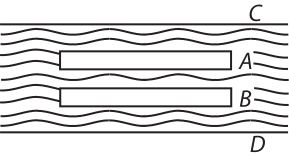
\includegraphics[width=0.3\textwidth]{images/35_5_7v1}\\\textit{[Fig. 4]}
                        %\caption{Bildbeschreibung}
           %             \end{wrapfigure}
                        %@ @ @ Dies ist eine Abstandszeile - fuer den Fall, dass mehrere figures hintereinander kommen, ohne dass dazwischen laengerer Text steht. Dies kann zu einer Fahlermeldung fuehren. @ @ @ \\
                     Manifestum est quod major erit celeritas\protect\index{Sachverzeichnis}{celeritas} inter \textit{A} et \textit{B}, quam inter \textit{A} et \textit{C}, et inter \textit{B} et \textit{D} quia eadem materia quae in obicis \textit{A} latitudinem impingit, aequaliter distribuetur in \edtext{intervalla}{\lemma{}\Afootnote{intervalla \textit{ erg.} \textit{ L}}} \textit{AC} et \textit{AD} et pars quae in \textit{B}, distribuetur aequaliter in intervalla \textit{BD} et \textit{BC}, jam quod tendit versus \textit{BC}, obsistit ei quod tendit versus \textit{AC}, necesse est igitur exitum in medio quaerere inter \textit{AB}. Hinc ergo impetus\protect\index{Sachverzeichnis}{impetus} fluminis conabitur utrumque rejicere in litus; et si alterum fixum sit, alterum tamen in ripam rejicietur, quae ratio est cur in fluminibus aut generaliter aquis fluctuantia paulatim rejiciantur in ripas; nam praesertim quod aliqua semper adsunt fixa; etiam illud considerandum est, ipsa fluctuantia aliquod habere fixitatis a pondere suo.
                     \pend
% Zeitz auskommentiert                    \begin{center}
%                      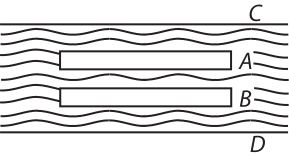
\includegraphics[width=0.4\textwidth]{images/35_5_7v1}\\\textit{[Fig. 6]}
%                      \end{center}
                      \pstart  
                      In superiore figura circularis motus considerandus est, quod pila\protect\index{Sachverzeichnis}{pila} in medio resistit nonnihil motui \textit{I} etiamsi gravis non sit, vel ideo quod inter movendum findit. Sed etsi non finderet (per impossibile) motus tamen ejus non fieret in instanti sed in tempore determinato. Moveretur enim celeritate\protect\index{Sachverzeichnis}{celeritas} quae ipsi imprimitur, nunc paulo minore.
                      \pend 
%    Zeitz auskommentiert                 \begin{center}
%                      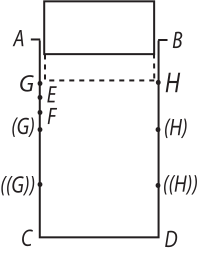
\includegraphics[width=0.3\textwidth]{images/35_5_7v2}\\\textit{[Fig. 7]}
%                      \end{center} 
                      \pstart Videndum autem an de Elaterio\protect\index{Sachverzeichnis}{elaterium} ratiocinari liceat, etiam sine ulla hypothesi. Nimirum ponamus vim oriri \edtext{a magnitudine}{\lemma{a}\Afootnote{ \textit{ (1) }\ quantitate \textit{ (2) }\ parvitate \textit{ (3) }\ magnitudine \textit{ L}}} materiae in spatio parvo, vel 
\edtext{a parvitate spatii}{\lemma{a}\Afootnote{ \textit{ (1) }\ magnitudine \textit{ (2) }\ parvitate spatii \textit{ L}}} pro materia \edtext{magna}{\lemma{materia}\Afootnote{ \textit{ (1) }\ parva \textit{ (2) }\ magna \textit{ L}}}. Erit ergo vis in reciproca spatiorum ratione. Ergo vis in \textit{GH}, erit ad vim in \textit{(G)(H)} ut est \textit{(G)C} ad \textit{GC}. Ergo vis  $\displaystyle (G)(H)$ $\sqcap$ vis $\displaystyle GH, \smallfrown \frac{GC}{(G)C}$ % \begin{wrapfigure}{l}{0.4\textwidth}                    
%                %\includegraphics[width=0.4\textwidth]{../images/Calculus+elasticus/LH035%2C05%2C02_007v/files/100246.png}
                        %\caption{Bildbeschreibung}
                        %\end{wrapfigure}
                        %@ @ @ Dies ist eine Abstandszeile - fuer den Fall, dass mehrere figures hintereinander kommen, ohne dass dazwischen laengerer Text steht. Dies kann zu einer Fahlermeldung fuehren. @ @ @ \\
                     et  vis  $\displaystyle((G))((H))$ $\sqcap$ vis $\displaystyle GH, \smallfrown \frac{GC}{((G))C}$% \begin{wrapfigure}{l}{0.4\textwidth}                    
                %\includegraphics[width=0.4\textwidth]{../images/Calculus+elasticus/LH035%2C05%2C02_007v/files/100248.png}
                        %\caption{Bildbeschreibung}
                        %\end{wrapfigure}
                        %@ @ @ Dies ist eine Abstandszeile - fuer den Fall, dass mehrere figures hintereinander kommen, ohne dass dazwischen laengerer Text steht. Dies kann zu einer Fahlermeldung fuehren. @ @ @ \\
                    , et \textit{(G)C} vel \textit{((G))C} appellando \textit{y}, \edtext{\textit{GC} appellando \textit{g}}{\lemma{\textit{y},}\Afootnote{ \textit{ (1) }\ fiet \textit{ (2) }\ et vim  \textit{(a)}\ \textit{GC} \textit{(b)}\ \textit{HG} appellando \textit{ (3) }\ \textit{GC} appellando \textit{g} \textit{ L}}}, \edtext{et vim \textit{GH} appellando \textit{v}}{\lemma{\textit{g},}\Afootnote{ \textit{ (1) }\ fiet, \textit{ (2) }\ et vim \textit{GH} appellando \textit{v} \textit{ L}}}, \edtext{et}{\lemma{\textit{v},}\Afootnote{ \textit{ (1) }\ fiet \textit{ (2) }\ et \textit{ L}}} vis generaliter erit: $vg \smallsmile y$. Vires ergo Elaterii aeris\protect\index{Sachverzeichnis}{elaterium!aeris} in quolibet puncto non ut alibi credideram per Hyperbolam cubicam, sed per Hyperbolam communem optime designantur. Jam de tempore restitutionis videndum est. Ponamus scilicet restitutionem fieri ex \textit{((G))((H))} et embolum\protect\index{Sachverzeichnis}{embolus} rejectum ex \textit{((G))((H))} pervenire in \textit{(G)(H)} tempore aliquo quod appellabimus \textit{t} quod infinite parvum ponemus,
  etiam spatio\protect\index{Sachverzeichnis}{spatium!infinite parvum} posito infinite \edtext{parvo. Porro embolus vi prima $vg \smallsmile ((G))C$ pervenit in \textit{[(G)(H)]},}{\lemma{parvo.}\Afootnote{ \textit{ (1) }\ Vis autem prima erit $vg \smallsmile ((G))C$, et vis secunda erit tum prima acquisita, tum praeterea secunda quae est: $vg \smallsmile ((G))C$. \textit{ (2) }\ Porro embolus vi prima $vg \smallsmile ((G))C$ pervenit [...] \textit{(G)H} \textit{ L}}} \edtext{at ex \textit{[(G)(H)]},}{\lemma{$(G)H$}\Afootnote{\textit{L ändert Hrsg.}}}
                     tendit altius vi tum quam habet ab \edtext{initio nempe $vg \smallsmile ((G))C$ tum quam}{\lemma{initio}\Afootnote{ \textit{ (1) }\ tum quam \textit{ (2) }\ nempe $vg \smallsmile (G)C$ tum quam \textit{ L}}} [nactus]\edtext{}{\Afootnote{nactum\textit{\ L \"{a}ndert Hrsg. } }} est \edtext{in itinere}{\lemma{est}\Afootnote{ \textit{ (1) }\ ab initio \textit{ (2) }\ in itinere \textit{ L}}} nempe $vg \smallsmile ((G))C + \gamma$. Spatium ergo \textit{(G)E} quod in secundo tempore percurret, 
                           erit ad spatium $((G))(G)\sqcap \gamma$ quod percurrit in primo, 
\edtext{ut $vg \smallsmile ((G))C + vg \smallsmile ((G))C [+] \gamma$}{\lemma{primo,}\Afootnote{ \textit{ (1) }\ ut $vg \smallsmile ((G))C$ ad \textit{ (2) }\ ut $vg \smallsmile ((G))C + vg \smallsmile ((G))C - \gamma$ \textit{ L ändert Hrsg.}}}
 %%%%%%%%%%%%%%%%%%%%%%%%%%%%%
% Zeitz auskommentiert
                    \edtext{seu spatium secundum \textit{(G)E} est}{\lemma{$vg \smallsmile ((G))C$}\Afootnote{ \textit{ (1) }\ seu est spat. sec. \textit{GE} $\sqcap$ \textit{ (2) }\ seu spatium secundum \textit{(G)E} est \textit{ L}}} 
\edtext{est ad $vg \smallsmile ((G))C$}{\lemma{$((G))C [+] \gamma$}\Afootnote{ \textit{ (1) }\ . Et porro vis quam percurrit in  \textit{(a)}\ secundo \textit{(b)}\ tertio temporis momento \textit{ (2) }\ est ad $vg \smallsmile ((G))C$ \textit{ L}}} 
%%%%%%%%%%%%%%%%%%%%%%%%%%%%%%%%%%%%
$\rule[-4mm]{0mm}{15mm}\displaystyle \sqcap \frac{\gamma \smallfrown \displaystyle\frac{vg}{((G))C}+\displaystyle\frac{vg}{((G))C+\gamma}}{\displaystyle\frac{vg}{((G))C}} 
\sqcap \gamma ((G)) C \smallfrown \frac{1}{((G))C}+\frac{1}{((G)) C + \gamma}$ 
sive [$\rule[-4mm]{0mm}{10mm}\displaystyle \frac{\gamma , ((G))C, 2 ((G)) C + \gamma}{((G))^2C^2 + \gamma}$]
%                   % \edtext{}{\Afootnote{$\displaystyle \frac{\gamma ((G)) C^3 + \gamma^2 ((G))C^2}{2 ((G)) C + \gamma}$ \textit{\ L \"{a}ndert Hrsg. } }}%
 \edtext{}{\lemma{$\displaystyle \frac{\gamma , ((G)) C, ((G)) C^2 + \gamma ((G)) C}{2 ((G)) C + \gamma}$}\Afootnote{  \textit{\ L \"{a}ndert Hrsg.}}}                   
sive: [$\displaystyle \frac{\gamma , 2 ((G))C +\gamma}{((G)) C + \gamma}$]. 
%
                    % \edtext{}{\Afootnote{$\displaystyle \frac{\gamma , ((G)) C,, ((G)) C^2 + \gamma ((G)) C}{2 ((G)) C + \gamma}$  \textit{\ L \"{a}ndert Hrsg. } }}
%
\edtext{}{\Afootnote{$\displaystyle \frac{\gamma ((G)) C^3 + \gamma^2 ((G))C^2}{2 ((G)) C + \gamma}$ \textit{\ L \"{a}ndert Hrsg.}}}%
 \edtext{In puncto autem \textit{E}}{\lemma{[$\displaystyle \frac{\gamma , 2 ((G))C + \gamma}{((G))C + \gamma}$].}\Afootnote{ \textit{ (1) }\ Spatium autem quod tertio tempore percurritur, nempe \textit{EF}, \textit{ (2) }\ In puncto autem \textit{E} \textit{ L}}} vim rursus acquirit novam, nempe: 
quae sit ad vim primam, $vg \smallsmile ((G))C$. ut est spatium \textit{((G))C} ad spatium \textit{EC}, seu ad spatium, [$\rule[-4mm]{0mm}{10mm}\displaystyle ((G)) C + \gamma + \gamma ((G))C \smallfrown \frac{1}{((G))C}+\frac{1}{((G))C + \gamma}$]\edtext{}{\Afootnote{$\displaystyle ((G))C + \gamma + \gamma((G))C \smallsmile \frac{1}{((G))C}+ \frac{1}{((G))C + \gamma}$ \textit{\ L \"{a}ndert Hrsg.}}}. 
Itaque spatium \textit{EF}, quod tertio tempore percurritur erit ad spatium $((G))(G) \sqcap \gamma$ primo tempore percursum, ut \edtext{est $\displaystyle 1 \smallsmile ((G))C + 1 \smallsmile ((G))C + \gamma, + 1 \smallsmile ((G))C + \gamma, + \gamma((G))C \smallfrown \frac{1}{((G))C}+\frac{1}{((G))C + \gamma}$ ad $\displaystyle \frac{1}{((G))C}$}{\lemma{est}\Afootnote{ \textit{ (1) }\ $\displaystyle 1 \smallsmile ((G))C + 1 \smallsmile ((G)) C + \gamma , + vg, \gamma , ((G))C \smallsmile \frac{1}{((G))C}+\frac{1}{((G))C + \gamma}$ ad \textit{v} \textit{ (2) }\ $\displaystyle 1 \smallsmile ((G))C + 1 \smallsmile ((G))C + \gamma , + 1 \smallsmile ((G))C + \gamma , + \gamma((G))C \smallfrown \frac{1}{((G))C}+\frac{1}{((G))C + \gamma}$ ad $\displaystyle \frac{1}{((G))C}$ \textit{ L}}}.
 Itaque spatium primo tempore percursum est $\gamma$ secundo \textit{(G)E} est $\displaystyle \gamma ((G))C \smallfrown \frac{1}{((G))C}+\frac{1}{((G))C + \gamma}$ tertio tempore percursum seu \textit{EF} est: 
%\edlabel{form0071}
[$\rule[-4mm]{0mm}{10mm}\displaystyle \gamma((G))C, \smallfrown \frac{1}{((G))C}+\frac{1}{((G))C+\gamma},, + \gamma((G))C, \smallfrown \frac{1}{((G))C + \gamma + \gamma((G))C, \smallfrown \displaystyle\frac{1}{((G))C}+\displaystyle\frac{1}{((G))C+ \gamma}}$] 
\edtext{\edlabel{form0072}}{\lemma{$\displaystyle \gamma ((G))C \smallfrown \frac{1}{((G))C}+\frac{1}{((G))C + \gamma},, + \gamma((G))C, \smallfrown \frac{1}{GC}+ \frac{1}{((G))C + \gamma}$}\xxref{form0071}{form0072}\Afootnote{ \textit{L \"{a}ndert Hrsg.}}}